\documentclass{article}
\usepackage[UTF8]{ctex}
\usepackage{amsmath}
\usepackage{amssymb}
\usepackage{amsthm}
\usepackage{graphicx}
\usepackage{marvosym}
\usepackage{xeCJKfntef}
\usepackage[hidelinks]{hyperref}

\bibliographystyle{plain}

\title{赛题二:离散高斯分布}
\author{程俊杰$^{\href{mailto:htk90uggk@outlook.com}{\textrm{\Letter}}}$}
\date{\today}

\begin{document}
    \maketitle
    \section{第一题}
    第一题的标准差$\sigma = 0.75$,中心为$c = 0$,$\pm5$的采样概率总共为$2.38 * 10^{-10}$,因此只在$[-4, 4]$中采样足够应付比赛。概率矩阵的前8列为:
    \begin{equation}
        \begin{pmatrix}
            1 & 0 & 0 & 0 & 1 & 0 & 0 & 0 \\
            0 & 1 & 1 & 0 & 1 & 1 & 1 & 1 \\
            0 & 0 & 0 & 0 & 0 & 1 & 1 & 1 \\
            0 & 0 & 0 & 0 & 0 & 0 & 0 & 0 \\
            0 & 0 & 0 & 0 & 0 & 0 & 0 & 0
        \end{pmatrix}
        \mbox{。}
    \end{equation}
    
    
    8比特随机数组成一个无符号数,有如下可能:
    \begin{enumerate}
        \item 0*******:取值范围为[0, 127),共128种可能,在概率矩阵的第一列采样成功,采样值为$\{0\}$;\label{uint8_t_1}
        \item 10******:取值范围为[128, 192),共64种可能,在概率矩阵的第二列采样成功,采样值为$\{1\}$;\label{uint8_t_2}
        \item 110*****:取值范围为[192, 224),共32种可能,在概率矩阵的第三列采样成功,采样值为$\{1\}$;\label{uint8_t_3}
        \item 1110****:取值范围为[224, 240),共16种可能,在概率矩阵的第五列采样成功,采样值为$\{0, 1\}$;\label{uint8_t_4}
        \item 11110***:取值范围为[240, 248),共8种可能,在概率矩阵的第六列采样成功,采样值为$\{1, 2\}$;\label{uint8_t_5}
        \item 111110**:取值范围为[248, 252),共4种可能,在概率矩阵的第七列采样成功,采样值为$\{1, 2\}$;\label{uint8_t_6}
        \item 1111110*:取值范围为[252, 254),共2种可能,在概率矩阵的第八列采样成功,采样值为$\{1, 2\}$;\label{uint8_t_7}
        \item 1111111*:取值范围为[254, 255],共2种可能,无法在概率矩阵的前八列采样成功。\label{uint8_t_8}
    \end{enumerate}
    首先看情况~\ref{uint8_t_1}~至~\ref{uint8_t_6},对于一个随机8比特无符号数,有:
    \begin{itemize}
        \item $128^{[\ref{uint8_t_1}]} + 16/2^{[\ref{uint8_t_4}]} = 136$种可能对应的采样值为0;
        \item $64^{[\ref{uint8_t_2}]} + 32^{[\ref{uint8_t_3}]} + 16/2^{[\ref{uint8_t_4}]} + 8/2^{[\ref{uint8_t_5}]} + 4/2^{[\ref{uint8_t_6}]} = 110$种可能对应的采样值为1;
        \item $8/2^{[\ref{uint8_t_5}]} + 4/2^{[\ref{uint8_t_6}]} = 6$种可能对应的采样值为2;
        \item 对于非0采样值,注意是$\pm i$共同的采样可能。
    \end{itemize}
    因此,维护一个长度为$136 + 110 + 6 = 252$的采样表,其中0的数量为136,$\pm1$的数量分别为55,$\pm2$的数量分别为3,则可以通过8比特随机数以$\frac{252}{256} = \frac{63}{64}$的概率直接查表得到采样值,而且是带正负号的。
    
    对于情况~\ref{uint8_t_7},若8比特无符号数为252,则认为采样值为1;若为253,则认为采样值为2,这两个数也存在采样表中。由于在第八列才采样成功,用尽了8比特无符号数中的所有随机比特,因此还需要一个额外的随机比特确定正负号。
    
    对于情况~\ref{uint8_t_8},继续运行Knuth-Yao算法直到采样成功。
    
    对于任意一个8比特随机数,其落在情况\ref{uint8_t_1}~至\ref{uint8_t_6}~的概率为$\frac{63}{64}$,称为关键路径,关键路径上的操作是影响采样速率最主要的因素。路径上的操作有:
    \begin{itemize}
        \item 获取随机数,随机数生成器存储了512字节的随机数,获取随机数实际上是一个查表操作,即访问一次内存;
        \item 根据随机数查采样表,访问一次内存,返回采样值;
        \item 由于这些内存需要经常访问,实际上是常驻缓存的。
    \end{itemize}
    这意味着关键路径已经被精简成两次缓存访问,一次采样共需要不到8个时钟周期(现代CPU的缓存命中延迟可以低至1-2个时钟周期,这里多出来的时钟周期应该是随机数填充、if判断、前8比特采样失败等情况所造成的。),这已经没办法继续优化了。
    
    一些理论上但实际不可行的优化:
    \begin{itemize}
        \item 减少获取随机数的时间:
        \begin{itemize}
            \item 直接放弃随机数,维护一个非常长的采样表samples以及一个计数器cnt,每次采样返回samples[cnt++]。可以将采样时间减少到4个时钟周期,但是采样多少次就需要事先存好多大的采样表,内存上不可行。
            \item 直接通过RDRAND指令获取硬件随机数,但是该指令安全性很高,类似于真随机数(是不是真随机数我也不清楚,但是这个指令跟CPU中的熵源有关系,Intel和AMD的熵源是什么我也没查),每获取一个随机数需要463个时钟周期,得不偿失。
            \item 自己实现一个更快的随机数生成器,但是官方给的随机数生成器速率每生成一个随机数大约只需要4个时钟周期,实现一个更快的可能性不大。
        \end{itemize}
        \item 减少访问采样表的时间:
        \begin{itemize}
            \item 直接通过随机数计算出采样值,但是计算随机数的指令也需要通过访问缓存获取、执行计算也需要时间,不如直接查采样表快。
        \end{itemize}
    \end{itemize}
    \textbf{不严谨}地说,任何超过2次内存(缓存)访问的算法,采样速度都不可能低至8个时钟周期。而获取随机数需要一次内存访问,得到对应的采样值至少需要一次内存访问,因此不存在内存访问次数小于2的采样算法。
    
    \textbf{时间复杂度}:8个时钟周期,主频为2.8GHz的PC上采样速率为$3.57*10^8$~样本/秒。
    
    \textbf{空间复杂度}:概率矩阵的行对应采样范围,列对应采样精度,5行24列的矩阵足够满足一亿次采样的精度。因此共需要$5 * (24-8)\mbox{(前8列无需存储)} + (24-8)\mbox{(列和向量)} + 254\mbox{(采样表)} = 390$字节的存储空间。
    

    \section{第二题}
    略。

    \section{第三题}
    对于给定离散半高斯分布 $D_{\mathbb{Z}^+, \sigma_{\mathrm{max}}}$,定义分布:
    \begin{equation}
        BG_{\sigma_{\mathrm{max}}}(z) = \frac{1}{2} 
        \begin{cases}
            D_{\mathbb{Z}^+, \sigma_{\mathrm{max}}}(-z) & z \leq 0 \\
            D_{\mathbb{Z}^+, \sigma_{\mathrm{max}}}(z - 1) & z \geq 1
        \end{cases}
        \mbox{。}
    \end{equation}
    使用$BG_{\sigma_{\mathrm{max}}}$采样$z_0$,计算$z = (2b - 1) \cdot z_0 + b$,并以概率$p = \exp(\frac{z_0^2}{2\sigma_{\mathrm{max}}^2} - \frac{(z - \mu)^2}{2\sigma^2} \CJKsout{- m})$输出$z$,则$z$服从$D_{\mathbb{Z}, \sigma, \mu}$,其中$b$为0-1随机数\CJKsout{,$m$为使得$p \in (0, 1)$的偏值},$p \leq 1$。

    \begin{equation}
        p = \frac{D_{\mathbb{Z}, \sigma, \mu}(z)}{BG_{\sigma_{\mathrm{max}}}(z)} = 
        \begin{cases}
            \exp(\frac{z^2}{2\sigma_{\mathrm{max}}^2} - \frac{(z - \mu)^2}{2\sigma^2}) & z \leq 0 \\
            \exp(\frac{(z - 1)^2}{2\sigma_{\mathrm{max}}^2} - \frac{(z - \mu)^2}{2\sigma^2}) & z \geq 1
        \end{cases}
         = \exp(\frac{z_0^2}{2\sigma_{\mathrm{max}}^2} - \frac{(z - \mu)^2}{2\sigma^2})
         \mbox{。}
    \end{equation}

    \begin{proof}
        已知$\sigma \leq \sigma_{\mathrm{max}}$且$\mu \in [0, 1)$。当$z \leq 0$时,有:
        \begin{equation*}
            \frac{z^2}{2\sigma_{\mathrm{max}}^2} \leq \frac{z^2}{2\sigma^2} \leq \frac{(z - \mu)^2}{2\sigma^2}
            \mbox{。}
        \end{equation*}
        当$z \geq 1$时,有:
        \begin{equation*}
            \frac{(z - 1)^2}{2\sigma_{\mathrm{max}}^2} \leq \frac{(z - 1)^2}{2\sigma^2} \leq \frac{(z - \mu)^2}{2\sigma^2}
            \mbox{。}
        \end{equation*}
        综上,有$p \leq 1$。
    \end{proof}

    Howe等人\cite{q3}给出了$D_{\mathbb{Z}^+, 1.8205}$各点的采样概率(怎么算出来的没看明白),使用该分布构造的$BG_{1.8205}$与第三题需要实现的概率分布拟合度较高,$m$取0.391790725992496即可满足要求,如图~\ref{fig:q3}~所示。
    \begin{figure}[htb]
        \centering
        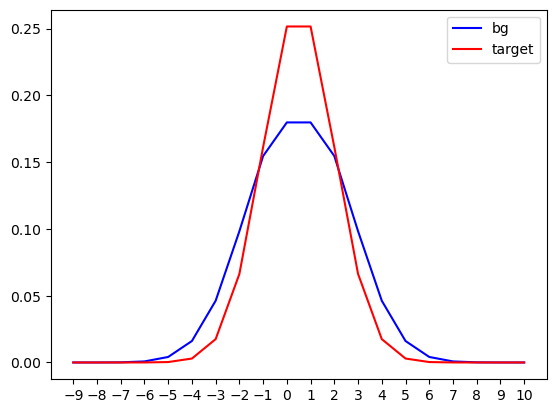
\includegraphics[width=.6\textwidth]{q3_0.5.png}
        \caption{$BG_{\sigma_{\mathrm{max}}}(z)$与目标分布}
        \label{fig:q3}
    \end{figure}

    由于有了$D_{\mathbb{Z}^+, 1.8205}$各点的采样概率,则可以直接使用第一题的采样算法实现,并在此基础上构造$BG_{1.8205}$和$D_{\mathbb{Z}, \sigma, \mu}$。

    \textbf{目前存在的问题}:
    \begin{enumerate}
        \item \CJKsout{$\mathrm{exp}(x)$使用Howe等人\cite{q3}给出的泰勒展开计算误差较大,采样结果无法通过卡方检测,使用数学库math则可以通过检测。但是奇怪的是math库也是泰勒展开近似的。}
        
        Howe等人给出的泰勒展开要求$x \in [-\ln(2), 0]$,然而实际上$x$经常远小于$-\ln(2)$,因此泰勒展开的误差较大。若$x < -\ln(2)$,则递归地计算$e^x = (e^{x/2})^2$,可以有效减小误差。

        \item $BG_{1.8205}$离目标分布还有一定的差距,如果能有更好的拟合,即图~\ref{fig:q3}~中的两条曲线更接近,那么拒绝采样率会更低。\CJKsout{可以预见,$BG_{1.7}$有更好的拟合度,但是我还求不来:(}。求不来是真的,但是还是别随便预见了。
    \end{enumerate}

    \section{第四题}
    使用第三题算法即可,略。

    \textbf{目前性能较低的部分}:
    \begin{enumerate}
        \item 计算$e^x$需要大量浮点数乘法,且为满足精度,目前为递归函数。
        \item $D_{\mathbb{Z}^+, 1.8205}$对于第三题和第四题来说可能不是非常合适,但是看不明白离散半高斯分布各点概率是怎么算的,只能用这个凑合。
    \end{enumerate}

    \bibliography{Sampler.bib}

    \appendix
    \newpage
    \section{第一题性能分析图}
    \begin{figure}[htb]
        \centering
        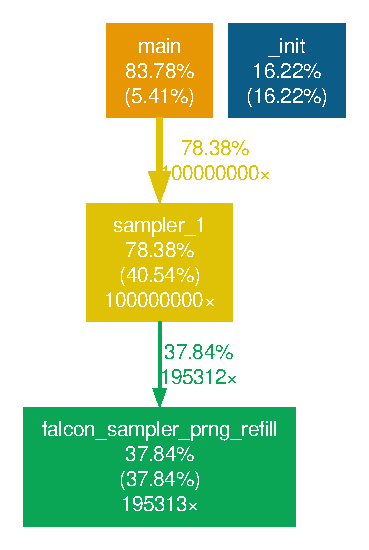
\includegraphics[width=.6\textwidth]{../gprof_figs/sampler_1.eps}
        \caption{第一题各函数运行时间占比}
    \end{figure}

    \section*{第三题性能分析图}
    \begin{figure}[htb]
        \centering
        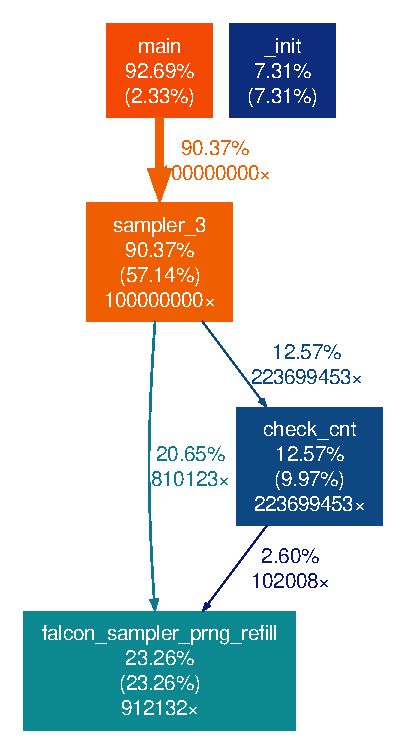
\includegraphics[width=.6\textwidth]{../gprof_figs/sampler_3.eps}
        \caption{第三题各函数运行时间占比}
    \end{figure}
\end{document}